
\section{Compositionality}





\begin{frame}{Meaning is built up}

\begin{itemize}
\item \txx{Compositional Semantics}: the meaning of the whole depends (only)
  on the meanings of the parts and the method of combination.
\item The hearer/reader's \txx{interpretation} brings in much more
  \begin{itemize}
  \item we bring in our existing knowledge
  \item we make inferences
  \end{itemize}
\item These inferences are based on (or constrained by) the semantics 
\item two central ideas \citep[formalized by: ][]{Katz:Fodor:1963}
  \begin{itemize}
  \item Semantic rules must be recursive to deal with infinite meaning
  \item Semantic rules interact with syntactic rules to build up meaning
  \end{itemize}
\item Two major components:
  \begin{itemize}
  \item A dictionary pairing lexical items with semantic representations
  \item A set of \txx{projection rules} that show how meaning is built up
  \end{itemize}
\end{itemize}

\end{frame}

\begin{frame}{Intersective Modification}

\begin{itemize}
\item Consider the simplest case of a noun and an adjective
  \begin{itemize}
  \item \lex{big} ``above average in size or number or quantity or magnitude or extent''
  \item \lex{head} ``the upper part of the human body or the front part of the body in animals; contains the face and brains''
  \end{itemize}
\item Each constrains the world, one picks out things that are
  ``big'' and the other things that ``are heads''.
\item Together \lex{big head} picks out things that have both properties: they
  are ``big'' and they ``have heads''.
\end{itemize}
\end{frame}

\begin{frame}{This is like intersection for sets}
\begin{center}
  \scalebox{2}{
    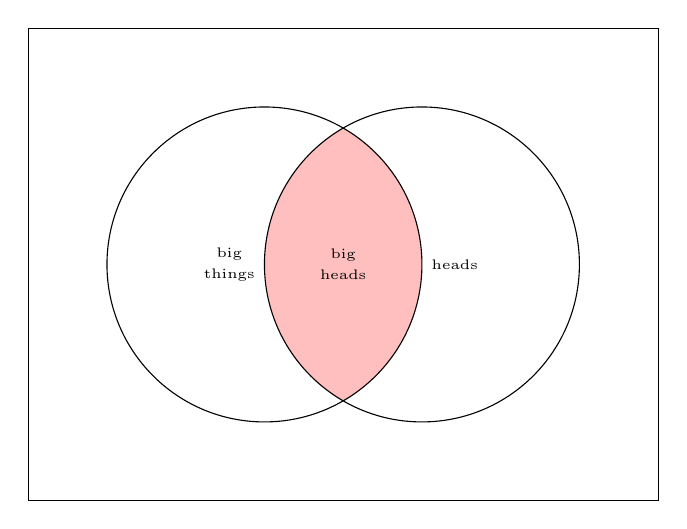
\begin{tikzpicture}
      \filldraw[fill=white] (-3,-3) rectangle (5, 3);
      \scope % A \cap B
      \clip (0,0) circle (2); \fill[pink] (2,0) circle (2);
      \endscope
      % outline
      \draw (0,0) circle (2) node [text=black,left,align=center] {\tiny\lex{big}\\ [-1ex] \tiny \lex{things}} 
      (2,0) circle (2) node [text=black,right] {\tiny\lex{heads}};
      \node[align=center] at (1,0) {\tiny \lex{big}\\[-1ex] \tiny \lex{heads}};
    \end{tikzpicture}} 
\end{center}

\begin{itemize}
\item This is the simplest form of composition
  \begin{itemize}
  \item although the meaning of big is not independent
  \end{itemize}
\end{itemize}

\end{frame}

\begin{frame}{Other kinds of intersective modification}

\begin{itemize}
\item \txx{Manner}: \eng{We \ull{live} very \ul{quietly}, sir} REDH
\item \txx{Restriction}: \eng{That trick of staining the fishes' scales of a delicate pink is quite \ull{peculiar} \ul{to China}} REDH
\item \txx{Location:} \eng{I would rather have my bracelets on him than on \ull{any criminal} \ul{in London}}
\item \txx{Time:} \eng{\ull{one day} \ul{in the autumn} \ul{of last year}}
\item \txx{State:} \eng{And \ull{sit} \ul{in the dark}}
\end{itemize}

The syntactic dependency (the fact that one word/phrase is associated
with another) helps us build the semantic model.  

\end{frame}

\begin{frame}{Some exceptions}

\begin{itemize}\addtolength{\itemsep}{-1ex}
\item Not all modification is intersective
  \begin{itemize}
  \item \eng{fake gun} is a thing like a gun: not a gun
  \item \eng{toy horse} is not a horse
  \item[?] come up with another example of non-intersective modification\task 
  \end{itemize}
  This requires different projection rules
\item Word combinations (\txx{multi-word expressions}) can pick up new
  meanings
  \begin{itemize}
  \item \eng{They have a big head} ``They are vain''
  \item \eng{They are a red head} ``They have red hair''
  \end{itemize}
  This requires a richer lexicon
\item There are many other ways of composing words (not just modification)
  \begin{itemize}
  \item Semantic roles: \eng{\ul{The dog} \ull{barked}}
  \item Intensification: \eng{They have a \ul{very} \ull{big} head}
  \item Embedding: \eng{I \ull{think} \ul{they have a big head}}
  \item Quantification: \eng{They have \ul{two} \ull{heads}/\ul{no} \ull{head}}
%  \item [\ldots]
  \end{itemize}
\end{itemize}

\end{frame}

%\begin{frame}{The dictionary}
% \MyLogo{Similar to \txx{genus} and \txx{differentiae}.}
% \begin{itemize}
% \item \lex{bachelor} \{N\}
%   \begin{enumerate}
%   \item \izb{human} \izb{male} [one who has never been married]
%   \item \izb{human} \izb{male} [young knight serving under the standard of another knight]
%   \item \izb{human} [one who has the lowest academic degree]
%   \item \izb{animal} \izb{male} [young fur seal without a mate in the breeding season]
%   \end{enumerate}
% \item \izb{semantic markers} are the links that bind lexical items
%   together in lexical relations
% \item {[\txx{distinguishers}]} serve to identify this particular lexical item
%     \\ this information is not relevant to syntax
% \end{itemize}

%\end{frame}

\begin{frame}{Projection Rules}
\MyLogo{More about this in Theories of Syntax/HPSG}

\begin{enumerate}
\item Projection rules combine with syntactic rules to produce the
  meaning of a sentence
  \\ these can be grouped together in \txx{signs} or \txx{constructions}
  \begin{itemize}
  \item Information is built up as we parse a sentence
    \begin{itemize}
    \item Information is only added, never deleted
    \item It must come from words or rules (or constructions)
    \end{itemize}
  \end{itemize}
\item Different languages show these combinations in different ways
  \begin{itemize}
  \item English primarily uses word order
  \item Japanese uses case-marking
  \item [\ldots{}]
  \end{itemize}
\item[?] Consider \eng{a very stout, florid-faced, elderly gentleman,
    with fiery red hair}
  \begin{itemize}
  \item How many examples of intersective modification are there here?\task
  \item Can you describe the other relations involved?\task
  \end{itemize}
  
% \item \txx{Selectional restrictions} \sr{} help to reduce ambiguity and
%   limit the possible readings
\end{enumerate}

\end{frame}

%\begin{frame}{Selectional restrictions} 

% \MyLogo{Modern theories prefer \txx{selectional preferences}:
%   probabilities not categories.}
% \begin{enumerate}
% \item \lex{colorful} \{adj\}
%   \begin{enumerate}
%   \item\label{A} \izb{color} [abounding in contract or variety of bright colors) 
%     \sr{\izb{physical object} or \izb{social activity}}
%   \item\label{B} \izb{evaluative} [having distinctive character, vividness or picturesqueness) 
%     \sr{\izb{aesthetic object} or \izb{social activity}}
%   \end{enumerate}

% \item \lex{ball} \{N\}
%   \begin{enumerate}
%   \item\label{D} \izb{social activity} \izb{large} \izb{assembly} [for the purpose of social dancing]
%   \item\label{E} \izb{physical object} [having globular shape]
%   \item\label{F} \izb{physical object} [solid missile for project by engine of war]
%   \end{enumerate}
% \end{enumerate}
% \begin{itemize}
% \item \eng{colorful ball}: The selectional restrictions rule out: \ref{B} $+$ \ref{E},  \ref{B} $+$ \ref{F}
% \end{itemize}

%\end{frame}

\begin{frame}{Completion}

\begin{itemize}
\item When we listen (or read) we actively anticipate the next word
  (or words)
\item We can guess them fairly well
  \begin{itemize}
\item \eng{Recognising, as I do, that you are the second highest
    expert in Europe-'}
\item \eng{'Indeed, sir! May I inquire who has the honour to be the
    first?' asked Holmes, with some asperity. \ldots}
  \item \eng{But as a practical man of affairs it is acknowledged that
      you stand alone. I trust, sir, that I have not inadvertently-'} ???
  \item \eng{'Just a little,' said Holmes. '}
  \end{itemize}
\item What is missing here?\task

\end{itemize}

\end{frame}
